\documentclass[12pt, a4paper]{report}
\usepackage[utf8]{inputenc}
\usepackage[english, russian]{babel}

\usepackage{graphicx}
\usepackage{listings}
\usepackage{color}

\usepackage{amsmath}
\usepackage{pgfplots}
\usepackage{url}
\usepackage{flowchart}
\usepackage{tikz}
\DeclareGraphicsExtensions{.pdf,.png,.jpg,.svg}
\usetikzlibrary{shapes, arrows}

\usepackage{pgfplotstable}

\renewcommand\contentsname{Содержание}

\usepackage{geometry}
\geometry{left=3cm}
\geometry{right=1cm}
\geometry{top=2cm}
\geometry{bottom=2cm}

\lstset{ %
language=C++,                 % выбор языка для подсветки (здесь это С)
basicstyle=\small\sffamily, % размер и начертание шрифта для подсветки кода
numbers=left,               % где поставить нумерацию строк (слева\справа)
numberstyle=\tiny,           % размер шрифта для номеров строк
stepnumber=1,                   % размер шага между двумя номерами строк
numbersep=-5pt,                % как далеко отстоят номера строк от         подсвечиваемого кода
backgroundcolor=\color{white}, % цвет фона подсветки - используем         \usepackage{color}
showspaces=false,            % показывать или нет пробелы специальными     отступами
showstringspaces=false,      % показывать или нет пробелы в строках
showtabs=false,             % показывать или нет табуляцию в строках
frame=single,              % рисовать рамку вокруг кода
tabsize=2,                 % размер табуляции по умолчанию равен 2 пробелам
captionpos=t,              % позиция заголовка вверху [t] или внизу [b] 
breaklines=true,           % автоматически переносить строки (да\нет)
breakatwhitespace=false, % переносить строки только если есть пробел
escapeinside={\%*}{*)},   % если нужно добавить комментарии в коде
keywordstyle=\color{blue}\ttfamily,
stringstyle=\color{red}\ttfamily,
commentstyle=\color{green}\ttfamily,
morecomment=[l][\color{magenta}]{\#},
columns=fullflexible }

\usepackage{titlesec}
\titleformat{\chapter}[hang]{\LARGE\bfseries}{\thechapter{.} }{0pt}{\LARGE\bfseries}
\titleformat*{\section}{\Large\bfseries}
\titleformat*{\subsection}{\large\bfseries}

\begin{document}

    \begin{titlepage}

        \begin{center}
            \Large
            {\sl Государственное образовательное учреждение высшего профессионального образования\\
            {\bf«Московский государственный технический университет имени Н.Э. Баумана»\\
				(МГТУ им. Н.Э. Баумана)}}
				\noindent\rule{\textwidth}{2pt}
            \vspace{3cm}

			{\scshape\LARGE Лабораторная работа №7 \par}
			\vspace{0.5cm}	
			{\scshape\LARGE по курсу «Анализ алгоритмов» \par}
			\vspace{1.5cm}
			{\huge\bfseries Поиск подстроки в строке \par}
			\vspace{2cm}
			\Large Выполнил: Сорокин А.П., гр. ИУ7-52Б\\
			\vspace{0.5cm}
			{\Large Преподаватели: Волкова Л.Л., Строганов Ю.В.}
		
			\vfill
			\Large \textit {Москва, 2019 г.}
            
        \end{center}

    \end{titlepage}
	
	\tableofcontents

	\chapter*{Введение}
	\addcontentsline{toc}{chapter}{Введение}
	
	\hspace{1cm}Поиск информации - одно из основных использований компьютера, и быстрый поиск точно заданной подстроки в строке является одной из самых простейших задач поиска информации. Однако эта задача является чрезвычайно важной. Данная функция встроена в различные текстовые редакторы и базы данных, что существенно ускоряет процесс поиска информации и редактирование фрагментов. В настоящее время функции поиска подстроки в строке инкапсулированы во многие высокоуровневые языки программирования. Но стоит помнить, что стандартные функции далеко не самые оптимальные и эффективные, и если основной задачей программы является нахождение подстроки в строке, то необходимо знать принципы организации функций поиска. Также не нужно забывать, что область применения функций поиска не ограничивается одними текстовыми редакторами и базами данных, наоборот, расширяется на различные сферы человеческой жизни.

    \chapter{Аналитическая часть}
	\section{Задачи}
	Цель лабораторной работы - изучение особенностей работы алгоритмов Кнута-Морриса-Пратта и Бойера-Мура.\\
	Для того чтобы добиться этой цели, были поставлены следующие задачи:
	\begin{itemize}
		\item применить знания программирования для реализации данных алгоритмов;
		\item получить практические навыки во время выполнения задания;
		\item экспериментально подтвердить различия во временной эффективности работы стандартного алгоритма поиска подстроки в строке, алгоритма Кнута-Морриса-Прата и Бойера-Мура.
	\end{itemize}

	\section{Описание алгоритмов}
	
	\subsection{Стандартный алгоритм}
	Стандартный алгоритм начинает со сравнения первого символа текста с первым символом подстроки. Если они совпадают, то происходит переход ко второму символу текста и подстроки. При совпадении сравниваются следующие символы. Так продолжается до тех пор, пока не окажется, что подстрока целиком совпала с отрезком текста, или пока не встретятся несовпадающие символы. В первом случае задача решена, во втором мы сдвигаем указатель текущего положения в тексте на один символ и заново начинаем сравнение с подстрокой \cite{macconnell}.
	
	\subsection{Алгоритм Кнута-Морриса-Пратта}
	Это — один из самых известных алгоритмов решения задачи поиска образца P в тексте T, имеющий временную оценку O(n), т. е. в нем поиск образца осуществляется за время, пропорциональное длине текста. В какой-то мере этот результат можно считать «точкой отсчета» в стремлении специалистов по информатике создать новые алгоритмы решения данной классической задачи. Здесь образец, как и в простом алгоритме, последовательно «прикладывается» к тексту и осуществляется пошаговое сравнение символов. Но если в простом алгоритме после несовпадения в какой-то позиции осуществляется сдвиг на одну позицию, то в рассматриваемом, за счет предварительного анализа P, сдвиг выполняется в некоторых случаях более чем на один символ, в отличие от стандартного алгоритма \cite{okulov}.
	
	\subsection{Алгоритм Бойера-Мура}
	Алгоритм Бойера-Мура осуществляет сравнение с образцом справа налево, а не слева направо. Исследуя искомый образец, можно осуществлять более эффективные прыжки в тексте при обнаружении несовпадения. В этом алгоритме кроме таблицы суффиксов применяется таблица стоп-символов. Она заполняется для каждого символа в алфавите. Для каждого встречающегося в подстроке символа таблица заполняется по принципу максимальной позиции символа в строке, за исключением последнего символа. При определении сдвига при очередном несовпадении строк, выбирается максимальное значение из таблицы суффиксов и стоп-символов\cite{macconnell}.
	
	\chapter{Конструкторская часть}
	
	В данном разделе представлены принципы работы алгоритмов и их схемы.
	На рисунках \ref{ris:first} и \ref{ris:kmp} представлен алгоритм Кнута-Морриса-Пратта.
	\begin{figure}[ht!]
		\centering
		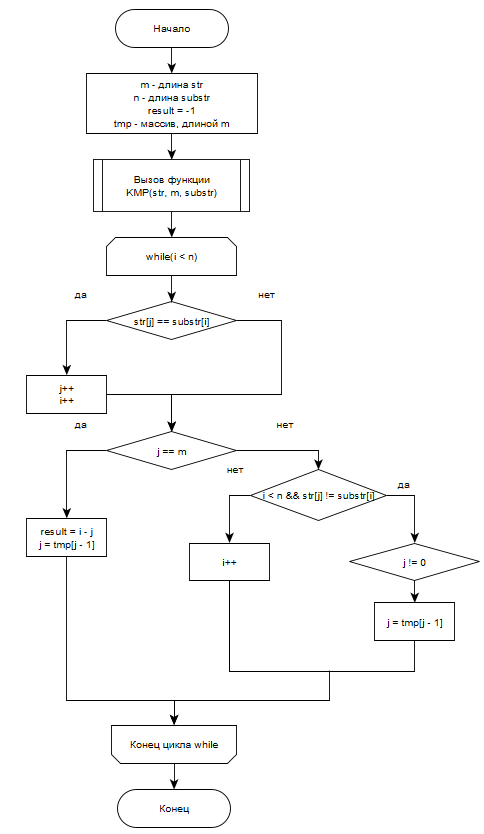
\includegraphics[scale=1.2]{img/first.png}
		\caption{Схема алгоритма Кнута-Морриса-Пратта}
		\label{ris:first}
	\end{figure}\newpage
	
	\begin{figure}[ht!]
		\centering
		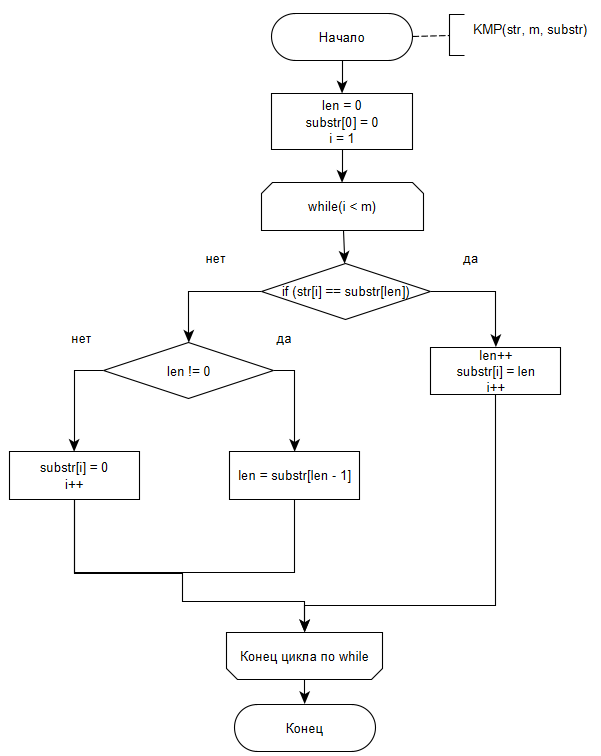
\includegraphics[scale=1.2]{img/kmp.png}
		\caption{Схема функции kmp}
		\label{ris:kmp}
	\end{figure}\newpage
	
	На рисунках \ref{ris:second} и \ref{ris:bad} представлен алгоритм Бойера-Мура.
	
	\begin{figure}[ht!]
		\centering
		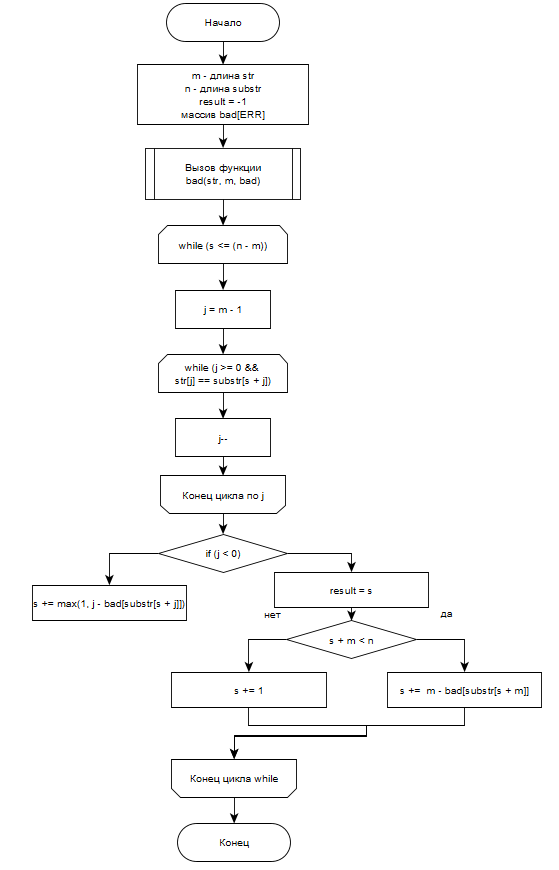
\includegraphics[scale=1.2]{img/second.png}
		\caption{Схема алгоритма Бойера-Мура}
		\label{ris:second}
	\end{figure}\newpage
	
	\begin{figure}[ht!]
		\centering
		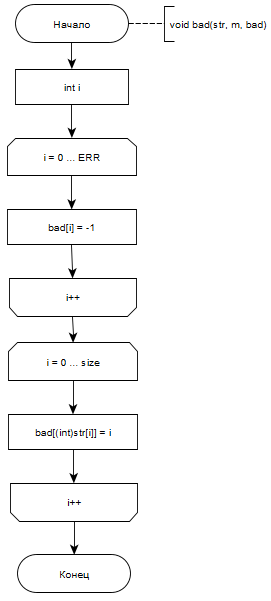
\includegraphics[scale=1.2]{img/bm.png}
		\caption{Схема функции bad}
		\label{ris:bad}
	\end{figure}\newpage

	\newpage
	
	\chapter{Технологическая часть}
	В данном разделе приведены требования к программному обеспечению, средствам реализации, а также листинги кода.
	\section{Средства реализации}
	Для реализации программы был использован язык C++ ~\cite{CPP}. Для замера процессорного времени была использована функция rdtsc() из библиотеки stdrin.h. Потоки реализовывались с использованием библиотеки pthreads.h.
	\section{Реализации алгоритмов}
	В листингах \ref{code-std}, \ref{code-kmp}, \ref{code-bm} представлен коды реализаций рассматриваемых в данной лабораторной работе алгоритмов поиска подстроки в строке.
	\begin{lstlisting}[label=code-std,caption=Стандартный алгоритм]
	int substr_std(std::string s, std::string subs)
	{
		int sn = s.length(), subn = subs.length();
		int n = sn - subn + 1;
	
		for (int i = 0; i < n; i++)
		{
			bool correct = true;
			for (int j = 0; j < subn && correct; j++)
				if (subs[j] != s[i + j])
					correct = false;
				if (correct)
					return i;
		}
		return -1;
	}
	\end{lstlisting}
	
	\begin{lstlisting}[label=code-kmp,caption=Алгоритм Кнута-Морриса-Пратта]
	void fail_compute(std::string s, int n, int *fail)
	{
		fail[0] = 0;
		for (int i = 1; i < n; i++)
		{
			int j = fail[i - 1];
			while (j > 0 && s[i] != s[j])
				j = fail[j - 1];
			if (s[i] == s[j])
				j++; 
			fail[i] = j;
		}
	}
	
	int substr_kmp(std::string s, std::string subs)
	{
		int sn = s.length(), subn = subs.length();
		int *fail = new int[subn];
	
		fail_compute(subs, subn, fail);
	
		int j = 0;
		for (int i = 0; i < sn; i++)
		{
			while (j > 0 && subs[j] != s[i])
				j = fail[j - 1];
			if (subs[j] == s[i])
				j++;
			if (j == subn)
			{
				delete [] fail;
				return i - subn + 1;
			}
		}
		delete [] fail;
		return -1;
	}
	\end{lstlisting}
	
	\begin{lstlisting}[label=code-bm,caption=Алгоритм Бойера-Мура]
	void bad(std::string subs, int size, int *badchar)
	{
		for (int i = 0; i < 256; i++)
			badchar[i] = -1;
		for (int i = 0; i < size; i++)
			badchar[(int)subs[i]] = i;
	}
	
	int substr_bm(std::string s, std::string subs)
	{
		int sn = s.length(), subn = subs.length();
		int result = -1;
		int badchar[SIZE];
		bad(subs, subn, badchar);
	
		int i = 0;
		while (i <= sn - subn)
		{
			int j = subn - 1;
			while (j >= 0 && subs[j] == s[i + j])
				j--;
			if (j < 0)
			{
				result = i;
				i += (i + subn < sn) ? subn - badchar[(int)s[i + subn]] : 1;
			}
			else
				i += std::max(1, j - badchar[(int)s[i + j]]);
		}
		return result;
	}
	\end{lstlisting}

	\newpage

	\section{Тесты}
	Для проверки корректности работы были подготовлены функциональные тесты, представленные в таблице \ref{unit-tests}.

	\begin{table}[ht!]
		\caption{Функциональные тесты}
		\label{unit-tests}
		\begin{center}
			\begin{tabular}{|c|c|c|}
			
			\end{tabular}
		\end{center}
	\end{table}

	В результате проверки реализации всех алгоритмов прошли тесты.

	\chapter{Экспериментальная часть}
	В данном разделе будет проведён сравнительный анализ реализаций стандартного алгоритма поиска подстроки в строке, алгоритма Кнута-Морриса-Пратта и Бойера-Мура.
	\section{Примеры работы}
	На рисунке \ref{pic:example} представлен пример работы программы, демонстрирующий корректную работу алгоритмов.
	\begin{figure}[ht!]
		\centering
		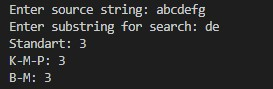
\includegraphics[scale=1]{img/example.jpg}
		\caption{Пример работы программы}
		\label{pic:example}
	\end{figure}
	
	\section{Сравнение работы алгоритмов}
	Для сравнения времени работы алгоритмов поиска подстроки в строке были использованы случайные строки длиной от 10 до 200 с шагом 10 и подстрока фиксированной длины 2. Эксперимент для более точного результата повторялся 100 раз. Итоговый результат рассчитывался как средний из полученных результатов. Результаты измерений показаны в таблице \ref{table-res} и на рисунке \ref{graph-res}.\\
	\begin{table}[ht!]
		\caption{Время работы алгоритмов поиска подстроки в строке в тактах процессора}
		\label{table-res}
		\begin{center}
			\pgfplotstabletypeset[
			col sep=semicolon,
			string type,
			columns/Size/.style={column name=Размер строки, column type={|c}},
			columns/Std/.style={column name=Стандартный, column type={|c}},
			columns/KMP/.style={column name=Алг-м Кнута-Морриса-Пратта, column type={|c}},
			columns/BM/.style={column name=Алг-м Бойера-Мура, column type={|c|}},
			every head row/.style={before row=\hline,after row=\hline},
			every last row/.style={after row=\hline},
			]{time.csv}
		\end{center}
	\end{table}

	\newpage
	
	\begin{figure}[ht!]
		\begin{tikzpicture}
		\begin{axis}
			[%title = График времени работы алгоритмов поиска подстроки в строке,
			table/col sep = semicolon,
			xlabel={Размер строки},
			ylabel={Время в тиках},
			ymin = 0,
			legend pos=outer north east,
			ymajorgrids=true,
			grid style=dashed]
			\addplot[color=red, mark=*] table[x={Size}, y={Std}] {time.csv};
			\addplot[color=blue, mark=*] table[x={Size}, y={KMP}] {time.csv};
			\addplot[color=green, mark=*] table[x={Size}, y={BM}] {time.csv};
			\legend{Стандартный алгоритм, Алгоритм Кнута-Морриса-Пратта, Алгоритм Бойера-Мура}
		\end{axis}
		\end{tikzpicture}
		\caption{График времени работы алгоритмов поиска подстроки в строке}
		\label{graph-res}
	\end{figure}
	
	Эксперименты показали, что наиболее эффективным алгоритмом из трех рассмотренных оказался стандартный алгоритм, а самым неэффективным оказался алгоритм Бойера-Мура.

	\chapter*{Заключение}
	\addcontentsline{toc}{chapter}{Заключение}
	В ходе выполнения данной лабораторной работы были изучены два алгоритма для поиск подстроки в строке - Кнута-Морриса-Пратта и Бойера-Мура. Во время разработки программного обеспечения были получены практические навыки реализации указанных алгоритмов.
	
	\newpage
	
	\begin{thebibliography}{}
	\bibitem{macconnell} Дж. Макконнелл. Анализ алгоритмов. Активный обучающий подход
	\bibitem{okulov} Окулов С.М. Алгоритмы обработки строк. – М.: БИНОМ. Лаборатория знаний, 2009.
	\bibitem{CPP} https://cppreference.com/ [Электронный ресурс]
	\end{thebibliography}
	\addcontentsline{toc}{chapter}{Литература}

\end{document}
